\documentclass{beamer}

\usepackage{moy-slides}
\usepackage{tikz}
\usepackage{comment}
\usepackage{listings}

\title[Path-focusing techniques]{Extension of Path-Focusing techniques}

%\subtitle{} % (optional)

\author[J. Henry, D. Monniaux, M. Moy]{Julien Henry, David Monniaux, Matthieu
Moy}
% - Use the \inst{?} command only if the authors have different
%   affiliation.

\newcommand{\important}[1]{\color{trefle}{#1}}

\institute[Verimag]{

\includegraphics[height=1.1cm]{../report/images/logoverimag}}

\tikzstyle{arrow}=[->,line width=.05cm,draw=red!90!blue!60!black]

\usetikzlibrary{fit}					% fitting shapes to coordinates
\usetikzlibrary{snakes,arrows,shapes,backgrounds,shadows,automata,patterns}
%\date{}
\usepgflibrary{snakes}

\tikzstyle{state}=[circle,fill=black!25,minimum size=13pt,inner sep=0pt]
\tikzstyle{transition}=[->,rectangle,thick,draw=black!75,
  			  fill=black!20,minimum size=4mm]
\tikzstyle{transition2}=[->,rectangle,thick,draw=blue!75,
  			  fill=blue,minimum size=4mm,blue]
\tikzstyle{PRstate}=[circle,fill=red!90,minimum size=13pt,inner sep=0pt]
\tikzstyle{polyhedra}=[blue!25,opacity=0.5,pattern=north west lines,pattern
color=blue]
\tikzstyle{line}=[black,thick]
\tikzstyle{NewPath}=[rectangle,thick,draw=black!75,
  			  fill=black!20,minimum size=4mm,dash pattern=on 3pt off 3pt]
\tikzstyle{TakenPath}=[rectangle,thick,draw=blue!75,
  			  fill=blue,minimum size=4mm,blue]


\begin{document}

\begin{frame}
  \titlepage
\end{frame}


\begin{frame}
\frametitle{Sources of imprecision in Abstract Interpretation}
\begin{itemize}
\item Abstract domain
\item \alert<2>{Widening operator}
\begin{itemize}
\item ensures fast convergence
\item BUT: may induce huge imprecisions
\item Narrowing tends to recover some precision\ldots
\end{itemize}
\item \alert<2>{Consider paths that are unfeasible in reality}
\end{itemize}
\end{frame}

\begin{frame}
\frametitle{Summary}
\tableofcontents
\end{frame}

\section[Introduction]{Introduction: Weakness of the standard approach}


\begin{frame}[containsverbatim]
  \frametitle{Example of standard Abstract Interpretation}
\begin{columns}
\begin{column}{5cm}
\begin{lstlisting}
x = 0;
y = 0;
while (true) {
	if (x <= 50) 
		y++;
	else 
		y--;

	if (y < 0) break;
	x++;
}
\end{lstlisting}
\end{column}
\begin{column}{5cm}
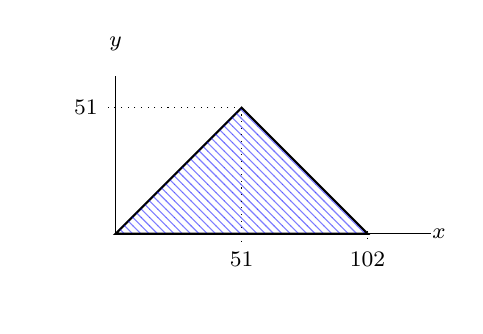
\begin{tikzpicture}[y=.2cm, x=.2cm,font=\footnotesize]

	\node (t1) at (-5,-4) {};
	\node (t2) at (13,11) {};
	\draw[line] (0,0) -- (8,8) -- (16,0) -- cycle;
	\fill[polyhedra] (0,0) -- (8,8) -- (16,0) -- cycle;
 	%axis
	\draw (0,0) -- coordinate (x axis mid) (20,0);
    \draw (0,0) -- coordinate (y axis mid) (0,10);

	%ticks and labels      
     		\draw [dotted](8,8) -- (-3pt,8) 
     			node[anchor=east] {$51$}; 
     		\draw [dotted] (8,8) -- (8,-3pt) 
     			node[anchor=north] {$51$}; 
     		\draw [dotted] (16,1pt) -- (16,-3pt) 
     			node[anchor=north] {$102$}; 

	\node[right=1.9cm] at (x axis mid) {$x$};
	\node[above=1.2cm] at (y axis mid) {$y$};
\end{tikzpicture} 
\end{column}
\end{columns}

\begin{itemize}
\item  $x$ and $y$ incremented during 51 iterations
\item  $x$ incremented and $y$ decremented during 51 iterations
\end{itemize}

\end{frame}

\begin{frame}
  \frametitle{Example of standard Abstract Interpretation}

\begin{columns}
  \begin{column}{6cm}
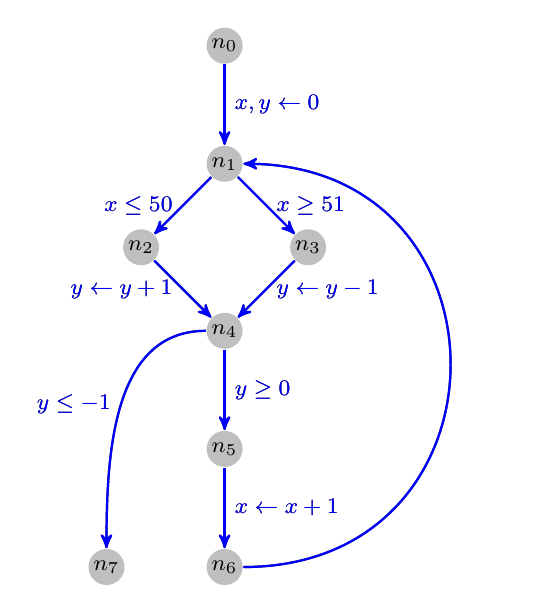
\begin{tikzpicture}[->,>=stealth',auto,node distance=1.5cm,
                    semithick,font=\footnotesize]

	\node[state] (n0) {$n_0$};
	\node[state] (n1) [below of=n0] {$n_1$};
	\node[state] (n2) [below left of=n1] {$n_2$};
	\node[state] (n3) [below right of=n1] {$n_3$};
	\node[state] (n4) [below left of=n3] {$n_4$};
	\node[state] (n5) [below of=n4] {$n_5$};
	\node[state] (n6) [below of=n5] {$n_6$};
	\node[state] (n7) [left of=n6] {$n_7$};

	\node (n8) [right of=n6] {};
	\node (n9) [right of=n1] {};

  \path<-1> [transition] 
		(n0) edge              node {$x,y \leftarrow 0$} (n1);
  \path<-2> [transition] 
        (n1) edge			   node [left] {$x \leq 50$} (n2);
  \path<-8> [transition] 
        (n1)  edge              node [right] {$x \geq 51$} (n3);
  \path<-3> [transition] 
        (n2) edge              node [left] {$y \leftarrow y+1$} (n4);
  \path<-9> [transition] 
        (n3) edge			   node [right] {$y \leftarrow y-1$} (n4);
  \path<-4> [transition] 
        (n4) edge			   node {$y \geq 0$} (n5);
  \path<-11> [transition] 
		(n4) edge  [out = 180, in=90] node [left] {$y \leq -1$} (n7);
  \path<-5> [transition] 
        (n5) edge              node {$x \leftarrow x+1$} (n6);
  \path<-6> [transition] 
        (n6) edge [out=0, in=0, distance=3.5cm] node {} (n1);

  \path<2-> [transition2] 
		(n0) edge              node {$x,y \leftarrow 0$} (n1);
  \path<3-> [transition2] 
        (n1) edge			   node [left] {$x \leq 50$} (n2);
  \path<9-> [transition2] 
        (n1)  edge              node [right] {$x \geq 51$} (n3);
  \path<4-> [transition2] 
        (n2) edge              node [left] {$y \leftarrow y+1$} (n4);
  \path<10-> [transition2] 
        (n3) edge			   node [right] {$y \leftarrow y-1$} (n4);
  \path<5-> [transition2] 
        (n4) edge			   node {$y \geq 0$} (n5);
  \path<12-> [transition2] 
		(n4) edge  [out = 180, in=90] node [left] {$y \leq -1$} (n7);
  \path<6-> [transition2] 
        (n5) edge              node {$x \leftarrow x+1$} (n6);
  \path<7-> [transition2] 
        (n6) edge [out=0, in=0, distance=3.5cm] node {} (n1);
\end{tikzpicture}
\end{column}
\begin{column}{5cm}
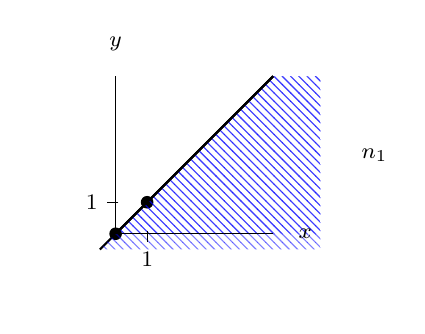
\begin{tikzpicture}[y=.2cm, x=.2cm,font=\footnotesize]

	\node (t1) at (-5,-4) {};
	\node (t2) at (13,11) {};
	\fill<2-7>[line] (0,0) circle (0.4);
	\fill<7>[line] (2,2) circle (0.4);
	\draw<8-10>[line] (0,0) -- (10,10) -- cycle;
	\draw<11-12>[line] (-1,-1) -- (10,10) -- cycle;
	\fill<11-12>[polyhedra] (-1,-1) -- (10,10) -- (13,10) -- (13,-1) -- (0,-1) -- cycle;
	\fill<13-14>[polyhedra] (0,0) -- (10,10) -- (13,10) -- (13,0) -- cycle;
	\draw<13-14>[line] (0,0) -- (10,10) -- cycle;

 	%axis
	\draw (0,0) -- coordinate (x axis mid) (10,0);
    \draw (0,0) -- coordinate (y axis mid) (0,10);

	%ticks and labels      
	\node[right=1.2cm] at (x axis mid) {$x$};
	\node[above=1.2cm] at (y axis mid) {$y$};

	\node[right=3cm] at (y axis mid) {$n_1$};

    \draw<7> (1pt,2) -- (-3pt,2) 
     	node[anchor=east] {1}; 
    \draw<7> (2,1pt) -- (2,-3pt) 
     	node[anchor=north] {1}; 

\end{tikzpicture} 
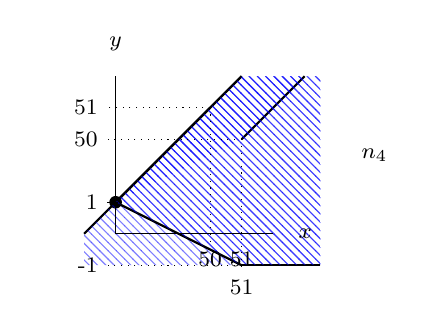
\begin{tikzpicture}[y=.2cm, x=.2cm,font=\footnotesize]

	\node (t1) at (-5,-4) {};
	\node (t2) at (13,11) {};
	\fill<4-9>[line] (0,2) circle (0.4);
	\fill<10-11>[polyhedra] (0,2) -- (8,10) -- (12,10) -- (8,6) --cycle;
	\draw<10-11>[line] (0,2) -- (6,8);
	\draw<10-11>[line] (8,6) -- (12,10);

	\draw<12-13>[line] (-2,0) -- (8,10);
	\fill<12-13>[polyhedra] (-2,-2) -- (-2,0) -- (8,10) -- (13,10) -- (13,-2) --
	 cycle;
	%\fill<12-13>[polyhedra] (-2,-2) -- (-2,0) -- (6,8) -- (6,-2) -- cycle;
	%\fill<12-14>[polyhedra] (8,6) -- (12,10) -- (13,10) -- (13,-2) -- (8,-2) -- cycle;

	\draw<14>[line] (0,2) -- (8,10);
	\draw<14>[line] (0,2) -- (8,-2);
	\draw<14>[line] (13,-2) -- (8,-2);
	\fill<14>[polyhedra] (0,2) -- (8,10) -- (13,10) -- (13,-2) -- (8,-2) -- cycle;
	%\fill<14>[polyhedra] (0,2) -- (6,8) -- (6,2) --  cycle;

 	%axis
	\draw (0,0) -- coordinate (x axis mid) (10,0);
    \draw (0,0) -- coordinate (y axis mid) (0,10);

	%labels      
	\node[right=1.2cm] at (x axis mid) {$x$};
	\node[above=1.2cm] at (y axis mid) {$y$};

	\node[right=3cm] at (y axis mid) {$n_4$};
	%ticks
     		\draw<4-> (1pt,2) -- (-3pt,2) 
     			node[anchor=east] {1}; 
     		\draw<14-> [dotted](8,-2) -- (-3pt,-2) 
     			node[anchor=east] {-1}; 
	
     		\draw<10-11> [dotted](6,8) -- (-3pt,8) 
     			node[anchor=east] {$51$}; 
     		\draw<10-11> [dotted] (8,6) -- (-3pt,6) 
     			node[anchor=east] {$50$}; 
     		\draw<10-11> [dotted](8,6) -- (8,-3pt) 
     			node[anchor=north] {$51$}; 
     		\draw<10-11> [dotted] (6,8) -- (6,-3pt) 
     			node[anchor=north] {$50$}; 
     		\draw<14-> [dotted](8,6) -- (8,-2.3) 
     			node[anchor=north] {$51$}; 
     		%\draw<14-> [dotted] (6,8) -- (6,-2.3) 
     		%	node[anchor=north] {$50$}; 
     		%\draw (2,1pt) -- (2,-3pt) 
     		%	node[anchor=north] {1}; 

\end{tikzpicture} 
\only<1-12>{Ascending iterations}
\only<13->{Descending iterations}
\end{column}
\end{columns}
\end{frame}

\begin{frame}
  \frametitle{Weakness of this approach}
	\begin{center}
		yields imprecision when a loop has several phases.
	\end{center}
\end{frame}

\section[Guided Static Analysis]{Guided Static Analysis}

\begin{frame}
  \frametitle{Principle}

D. Gopan \& T. Reps, CAV 2006
\bigskip
\begin{itemize}
\item separate loops into distinct phases.
\item obtaining a solution for each loop phase before proceeding to the next.
\item widening \& narrowing at each loop phase.
\begin{itemize}
\item Better precision
\end{itemize}
\end{itemize}
\end{frame}

\begin{frame}
\frametitle{Example}

\begin{columns}
  \begin{column}{6cm}
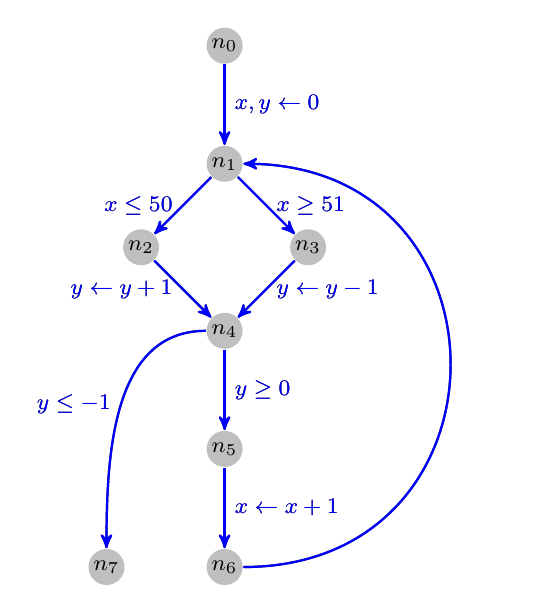
\begin{tikzpicture}[->,>=stealth',auto,node distance=1.5cm,
                    semithick,font=\footnotesize]

	\node[state] (n0) {$n_0$};
	\node[state] (n1) [below of=n0] {$n_1$};
	\node[state] (n2) [below left of=n1] {$n_2$};
	\node[state] (n3) [below right of=n1] {$n_3$};
	\node[state] (n4) [below left of=n3] {$n_4$};
	\node[state] (n5) [below of=n4] {$n_5$};
	\node[state] (n6) [below of=n5] {$n_6$};
	\node[state] (n7) [left of=n6] {$n_7$};

	\node (n8) [right of=n6] {};
	\node (n9) [right of=n1] {};

  \path<-1> [transition] 
		(n0) edge              node {$x,y \leftarrow 0$} (n1);
  \path<-2> [transition] 
        (n1) edge			   node [left] {$x \leq 50$} (n2);
  \path<-9> [transition] 
        (n1)  edge              node [right] {$x \geq 51$} (n3);
  \path<-3> [transition] 
        (n2) edge              node [left] {$y \leftarrow y+1$} (n4);
  \path<-10> [transition] 
        (n3) edge			   node [right] {$y \leftarrow y-1$} (n4);
  \path<-4> [transition] 
        (n4) edge			   node {$y \geq 0$} (n5);
  \path<-12> [transition] 
		(n4) edge  [out = 180, in=90] node [left] {$y \leq -1$} (n7);
  \path<-5> [transition] 
        (n5) edge              node {$x \leftarrow x+1$} (n6);
  \path<-6> [transition] 
        (n6) edge [out=0, in=0, distance=3.5cm] node {} (n1);

  \path<2-> [transition2] 
		(n0) edge              node {$x,y \leftarrow 0$} (n1);
  \path<3-> [transition2] 
        (n1) edge			   node [left] {$x \leq 50$} (n2);
  \path<10-> [transition2] 
        (n1)  edge              node [right] {$x \geq 51$} (n3);
  \path<4-> [transition2] 
        (n2) edge              node [left] {$y \leftarrow y+1$} (n4);
  \path<11-> [transition2] 
        (n3) edge			   node [right] {$y \leftarrow y-1$} (n4);
  \path<5-> [transition2] 
        (n4) edge			   node {$y \geq 0$} (n5);
  \path<13-> [transition2] 
		(n4) edge  [out = 180, in=90] node [left] {$y \leq -1$} (n7);
  \path<6-> [transition2] 
        (n5) edge              node {$x \leftarrow x+1$} (n6);
  \path<7-> [transition2] 
        (n6) edge [out=0, in=0, distance=3.5cm] node {} (n1);
\end{tikzpicture}
\end{column}
\begin{column}{5cm}
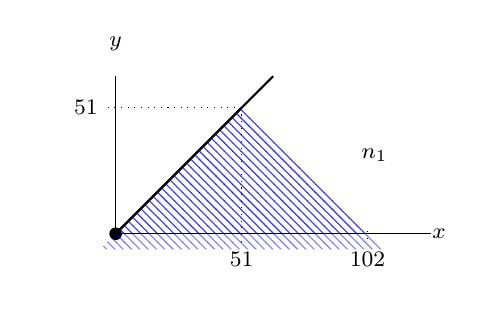
\begin{tikzpicture}[y=.2cm, x=.2cm,font=\footnotesize]

	\node (t1) at (-5,-4) {};
	\node (t2) at (13,11) {};
	\fill<2-6>[line] (0,0) circle (0.4);
	\draw<7-8>[line] (0,0) -- (10,10) -- cycle;
	\draw<9->[line] (0,0) -- (8,8) -- cycle;
	
	\fill<12-13>[polyhedra] (-1,-1) -- (8,8) -- (17,-1) -- cycle;
	\fill<14->[polyhedra] (0,0) -- (8,8) -- (16,0) -- cycle;
	
	%\draw<10-11>[line] (-1,-1) -- (10,10) -- cycle;
	%\fill<10-11>[polyhedra] (-1,-1) -- (10,10) -- (13,10) -- (13,-1) -- (0,-1) -- cycle;
	%\fill<12-13>[polyhedra] (0,0) -- (10,10) -- (13,10) -- (13,0) -- cycle;
	%\draw<12-13>[line] (0,0) -- (10,10) -- cycle;

 	%axis
	\draw (0,0) -- coordinate (x axis mid) (20,0);
    \draw (0,0) -- coordinate (y axis mid) (0,10);

	%ticks and labels      
     		\draw<9-> [dotted](8,8) -- (-3pt,8) 
     			node[anchor=east] {$51$}; 
     		\draw<9-> [dotted] (8,8) -- (8,-3pt) 
     			node[anchor=north] {$51$}; 
     		\draw<12-> [dotted] (16,1pt) -- (16,-3pt) 
     			node[anchor=north] {$102$}; 

	\node[right=1.9cm] at (x axis mid) {$x$};
	\node[above=1.2cm] at (y axis mid) {$y$};

	\node[right=3cm] at (y axis mid) {$n_1$};
\end{tikzpicture} 
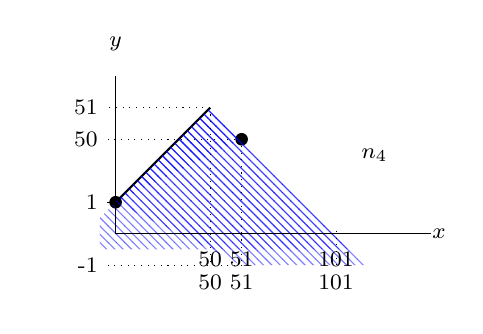
\begin{tikzpicture}[y=.2cm, x=.2cm,font=\footnotesize]

	\node (t1) at (-5,-4) {};
	\node (t2) at (13,11) {};
	\fill<4-7>[line] (0,2) circle (0.4);
	\draw<8->[line] (0,2) -- (6,8);
	
	\fill<11-12>[circle] (8,6) circle (0.4);
	\fill<11-12>[polyhedra] (8,6) -- (6,8) -- (0,2) -- cycle;

	\fill<13-14>[polyhedra] (6,8) -- (15,-1) -- (-1,-1) -- (-1,1) -- (0,2) -- cycle;
	\fill<15->[polyhedra] (6,8) -- (16,-2) -- (8,-2) -- (0,2) -- cycle;
	%\draw<11-12>[line] (-2,0) -- (8,10);
	%\fill<11-12>[polyhedra] (-2,-1) -- (-2,0) -- (8,10) -- (13,10) -- (13,-1) --
	% cycle;
	%\fill<11-12>[polyhedra] (-2,-1) -- (-2,0) -- (6,8) -- (6,-1) -- cycle;
	%\fill<11-13>[polyhedra] (8,6) -- (12,10) -- (13,10) -- (13,-1) -- (8,-1) -- cycle;

	%\draw<13-13>[line] (0,2) -- (8,10);
	%\draw<13-13>[line] (0,2) -- (8,-1);
	%\fill<13-13>[polyhedra] (0,2) -- (8,10) -- (13,10) -- (13,-1) -- (8,-1) -- cycle;
	%\fill<13-13>[polyhedra] (0,2) -- (6,8) -- (6,2) --  cycle;

 	%axis
	\draw (0,0) -- coordinate (x axis mid) (20,0);
    \draw (0,0) -- coordinate (y axis mid) (0,10);

	%labels      
	\node[right=1.9cm] at (x axis mid) {$x$};
	\node[above=1.2cm] at (y axis mid) {$y$};

	\node[right=3cm] at (y axis mid) {$n_4$};
	%ticks
     		\draw<4-> (1pt,2) -- (-3pt,2) 
     			node[anchor=east] {1}; 
     		\draw<15-> [dotted] (8,-2) -- (-3pt,-2) 
     			node[anchor=east] {-1}; 
     		\draw<8-> [dotted](6,8) -- (-3pt,8) 
     			node[anchor=east] {$51$}; 
     		\draw<8-14> [dotted] (6,8) -- (6,-3pt) 
     			node[anchor=north] {$50$}; 
     		\draw<15-> [dotted] (6,8) -- (6,-2) 
     			node[anchor=north] {$50$}; 
     		\draw<11-12> [dotted] (8,6) -- (-3pt,6) 
     			node[anchor=east] {$50$}; 
     		\draw<11-12> [dotted](8,6) -- (8,-3pt) 
     			node[anchor=north] {$51$}; 
     		\draw<15-> [dotted](8,0) -- (8,-2) 
     			node[anchor=north] {$51$}; 
     		\draw<13-14> [dotted] (14,1pt) -- (14,-3pt) 
     			node[anchor=north] {$101$}; 
     		\draw<15-> [dotted] (14,1pt) -- (14,-2) 
     			node[anchor=north] {$101$}; 
     		%\draw (2,1pt) -- (2,-3pt) 
     		%	node[anchor=north] {1}; 

\end{tikzpicture} 
\only<1-8>{Ascending iterations}
\only<10-13>{Ascending iterations}
\only<9>{Descending iterations}
\only<14->{Descending iterations}
\end{column}
\end{columns}
\end{frame}

\section[Path focusing]{Using SMT-solving to focus new paths}

\begin{frame}
  \frametitle{Principle}

D. Monniaux \& L. Gonnord
\bigskip
\begin{itemize}
\item Compute the fixpoint iterations on a multigraph
\item Take a set $P_R$ of nodes
\item Distinguish all the paths between 2 nodes of $P_R$
\end{itemize}
\bigskip
\visible<2>{
Exponential number of paths:
\begin{itemize}
\item We don't construct this graph explicitly
\item We use SMT-solving to find interesting paths
\end{itemize}
}
\end{frame}

\begin{frame}
  \frametitle{Reducing the graph}

\begin{columns}
\begin{column}{5.5cm}
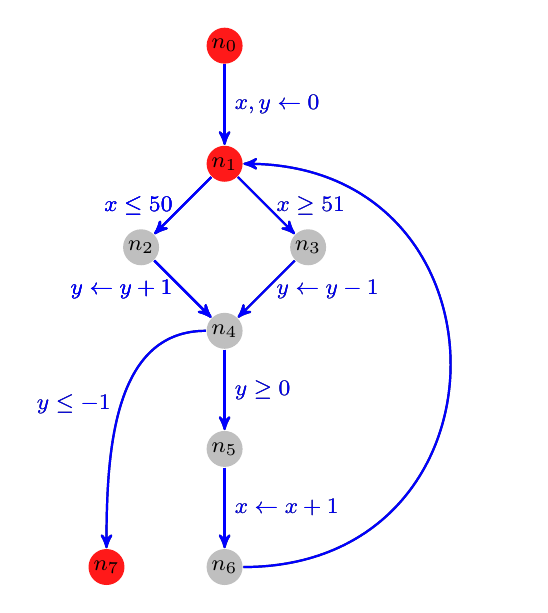
\begin{tikzpicture}[->,>=stealth',auto,node distance=1.5cm,
                    semithick,font=\footnotesize]

	\node[PRstate] (n0) {$n_0$};
	\node[PRstate] (n1) [below of=n0] {$n_1$};
	\node[state] (n2) [below left of=n1] {$n_2$};
	\node[state] (n3) [below right of=n1] {$n_3$};
	\node[state] (n4) [below left of=n3] {$n_4$};
	\node[state] (n5) [below of=n4] {$n_5$};
	\node[state] (n6) [below of=n5] {$n_6$};
	\node[PRstate] (n7) [left of=n6] {$n_7$};


  \path [transition] 
		(n0) edge              node {$x,y \leftarrow 0$} (n1);
  \path [transition] 
        (n1) edge			   node [left] {$x \leq 50$} (n2);
  \path [transition] 
        (n1)  edge              node [right] {$x \geq 51$} (n3);
  \path [transition] 
        (n2) edge              node [left] {$y \leftarrow y+1$} (n4);
  \path [transition] 
        (n3) edge			   node [right] {$y \leftarrow y-1$} (n4);
  \path [transition] 
        (n4) edge			   node {$y \geq 0$} (n5);
  \path [transition] 
		(n4) edge  [out = 180, in=90] node [left] {$y \leq -1$} (n7);
  \path [transition] 
        (n5) edge              node {$x \leftarrow x+1$} (n6);
  \path [transition] 
        (n6) edge [out=0, in=0, distance=3.5cm] node {} (n1);

  \path<3> [transition2] 
		(n0) edge              node {$x,y \leftarrow 0$} (n1);

  \path<4> [transition2] 
        (n1) edge			   node [left] {$x \leq 50$} (n2);
  \path<4> [transition2] 
        (n2) edge              node [left] {$y \leftarrow y+1$} (n4);
  \path<4-5> [transition2] 
        (n4) edge			   node {$y \geq 0$} (n5);
  \path<4-5> [transition2] 
        (n5) edge              node {$x \leftarrow x+1$} (n6);
  \path<4-5> [transition2] 
        (n6) edge [out=0, in=0, distance=3.5cm] node {} (n1);

  \path<5-6> [transition2] 
        (n1)  edge              node [right] {$x \geq 51$} (n3);
  \path<5-6> [transition2] 
        (n3) edge			   node [right] {$y \leftarrow y-1$} (n4);
  \path<6-> [transition2] 
		(n4) edge  [out = 180, in=90] node [left] {$y \leq -1$} (n7);

  \path<7> [transition2] 
        (n1) edge			   node [left] {$x \leq 50$} (n2);
  \path<7> [transition2] 
        (n2) edge              node [left] {$y \leftarrow y+1$} (n4);

\end{tikzpicture}
\end{column}
\begin{column}{5.5cm}
\visible<2->{
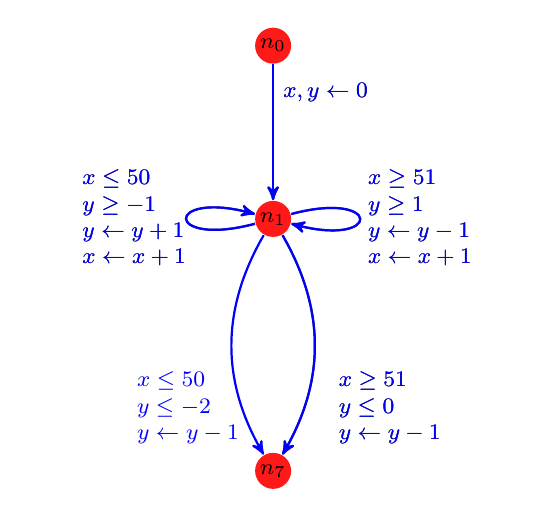
\begin{tikzpicture}[->,>=stealth',auto,node distance=3.2cm,
                    semithick,font=\footnotesize]

	\node[PRstate] (n0) {$n_0$};
	\node[PRstate] (n1) [below of=n0,yshift=1cm] {$n_1$};
	\node[PRstate] (n7) [below of=n1] {$n_7$};

	\node (n8) at (-3,0) {};
	\node (n8) at (3,0) {};

  \path<4-> [transition] 
		(n0) edge              node [yshift=5mm] {$x,y \leftarrow 0$} (n1);
  \path<7-> [transition] 
		(n1) edge    [bend left]  node [right,yshift=-0.8cm]  {$
		\begin{array}{l}
			x \geq 51 \\
			y \leq 0 \\
			y \leftarrow y-1
		\end{array}
		$} (n7);
%  \path<8-> [transition] 
%		(n1) edge    [bend right]  node [left,yshift=-0.8cm,xshift=4mm] {$
%		\begin{array}{l}
%			x \leq 50 \\
%			y \leq -2 \\
%			y \leftarrow y-1
%		\end{array}
%		$} (n7);
  \path<5-> [transition] 
		(n1) edge    [loop left,distance=1.2cm]  node [left,xshift=3mm] {$
		\begin{array}{l}
			x \leq 50 \\
			y \geq -1 \\
			y \leftarrow y+1 \\
			x \leftarrow x+1 
		\end{array}
		$} (n1);
  \path<6-> [transition] 
		(n1) edge    [loop right,distance=1.2cm]  node [right,xshift=-2mm] {$
		\begin{array}{l}
			x \geq 51 \\
			y \geq 1 \\
			y \leftarrow y-1 \\
			x \leftarrow x+1 
		\end{array}
		$} (n1);
  %\path [transition] 
  %      (n6) edge [out=0, in=0, distance=3.5cm] node {} (n1);
  \path<3> [transition2] 
		(n0) edge              node [yshift=5mm] {$x,y \leftarrow 0$} (n1);
  \path<6> [transition2] 
		(n1) edge    [bend left]  node [right,yshift=-0.8cm]  {$
		\begin{array}{l}
			x \geq 51 \\
			y \leq 0 \\
			y \leftarrow y-1
		\end{array}
		$} (n7);
  \path<7> [transition2] 
		(n1) edge    [bend right]  node [left,yshift=-0.8cm,xshift=4mm] {$
		\begin{array}{l}
			x \leq 50 \\
			y \leq -2 \\
			y \leftarrow y-1
		\end{array}
		$} (n7);
  \path<4> [transition2] 
		(n1) edge    [loop left,distance=1.2cm]  node [left,xshift=3mm] {$
		\begin{array}{l}
			x \leq 50 \\
			y \geq -1 \\
			y \leftarrow y+1 \\
			x \leftarrow x+1 
		\end{array}
		$} (n1);
  \path<5> [transition2] 
		(n1) edge    [loop right,distance=1.2cm]  node [right,xshift=-2mm] {$
		\begin{array}{l}
			x \geq 51 \\
			y \geq 1 \\
			y \leftarrow y-1 \\
			x \leftarrow x+1 
		\end{array}
		$} (n1);
\end{tikzpicture}
}
\end{column}
\end{columns}
\end{frame}

\begin{frame}
  \frametitle{Using SMT-solving to find new paths}
\begin{itemize}
\item SMT formula $\rho$ expressing the semantics of the program
\begin{itemize}
\item SMT: boolean + linear arithmetic
\end{itemize}
\item $\rho$ contains reachability predicates
\end{itemize}
\bigskip
``Does it exist a path starting in the invariant candidate, that arrives in a
state outside the invariant {?}`` 
\bigskip

$$f(p_i) = \rho \wedge b_i^s \wedge 
\displaystyle\bigwedge_{j \in P_R \atop j \neq i} \neg
b_j^s \wedge X_i \wedge \displaystyle\bigvee_{j \in Succ(i)} (b_j^d \wedge
 \neg X_j)$$


\footnotesize{
$b_{i}$: reachability predicate for $p_i$

$X_{i}$: abstract domain of node $p_i$
}
\end{frame}

\begin{frame}[containsverbatim]
	\frametitle{Example}
\begin{center}
\begin{lstlisting}
	int x = 0;
	int d = 1;
	
	while (true) {
		if (x == 0) d=1;
		if (x == 1000) d=-1;
		x +=d;
	}
\end{lstlisting}
\end{center}
\begin{itemize}
\item $x$ incremented until it is equal to $1000$,
\item $x$ decremented until it is equal to $0$,
\item restart\ldots
\end{itemize}

\end{frame}

\begin{frame}
  \frametitle{Example}
\begin{columns}
\begin{column}{7cm}
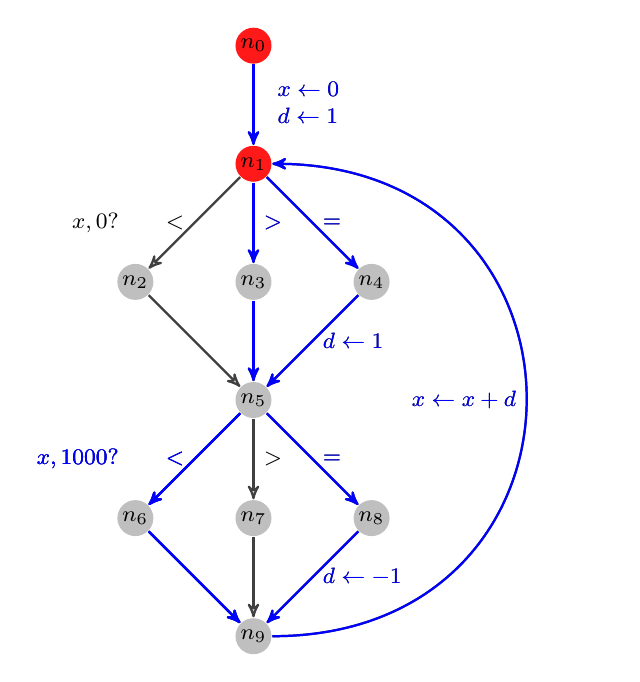
\begin{tikzpicture}[->,>=stealth',auto,node distance=1.5cm,
                    semithick,font=\footnotesize]
	\node[PRstate] (n0) {$n_0$};
	\node[PRstate] (n1) [below of=n0] {$n_1$};
	\node[state] (n3) [below of=n1] {$n_3$};
	\node[state] (n2) [left of=n3] {$n_2$};
	\node[state] (n4) [right of=n3] {$n_4$};
	\node[state] (n5) [below of=n3] {$n_5$};
	\node[state] (n7) [below of=n5] {$n_7$};
	\node[state] (n6) [left of=n7] {$n_6$};
	\node[state] (n8) [right of=n7] {$n_8$};
	\node[state] (n9) [below of=n7] {$n_9$};

  \path [transition] 
		(n0) edge              node  {$\begin{array}{l}
		x \leftarrow 0 \\
		d \leftarrow 1 
		\end{array}$} (n1);
  \path [transition] 
        (n1) edge			   node [left] {$x,0?$~ ~ ~ $<$} (n2);
  \path [transition] 
        (n1)  edge              node {$>$} (n3);
  \path [transition] 
        (n1)  edge              node [right] {$=$} (n4);
  \path [transition] 
        (n3) edge              node  {} (n5);
  \path [transition] 
        (n2) edge			   node {} (n5);
  \path [transition] 
        (n4) edge			   node [right] {$d \leftarrow 1$} (n5);
  \path [transition] 
        (n5) edge			   node [left] {$x,1000?$ ~ ~ ~$<$} (n6);
  \path [transition] 
        (n5) edge			   node {$>$} (n7);
  \path [transition] 
        (n5) edge			   node [right] {$=$} (n8);
  \path [transition] 
        (n6) edge              node {} (n9);
  \path [transition] 
        (n7) edge              node {} (n9);
  \path [transition] 
        (n8) edge              node [right] {$d \leftarrow -1$} (n9);
  \path [transition] 
        (n9) edge [out=0, in=0, distance=4.3cm] node [left] {$x \leftarrow x+d$} (n1);

  \path<1> [transition2] 
		(n0) edge              node  {$\begin{array}{l}
		x \leftarrow 0 \\
		d \leftarrow 1 
		\end{array}$} (n1);

  \path<2-3> [transition2] 
        (n1)  edge              node [right] {$=$} (n4);
  \path<2-3> [transition2] 
        (n4) edge			   node [right] {$d \leftarrow 1$} (n5);
  \path<2-5> [transition2] 
        (n5) edge			   node [left] {$x,1000?$ ~ ~ ~$<$} (n6);
  \path<2-5> [transition2] 
        (n6) edge              node {} (n9);
  \path<2-> [transition2] 
        (n9) edge [out=0, in=0, distance=4.3cm] node [left] {$x \leftarrow x+d$} (n1);
  \path<4-8> [transition2] 
        (n1) edge			   node {$>$} (n3);
  \path<4-8> [transition2] 
        (n3) edge			   node {} (n5);
	
  \path<6-7> [transition2] 
        (n5) edge			   node [right] {$=$} (n8);
  \path<6-7> [transition2] 
        (n8) edge              node [right] {$d \leftarrow -1$} (n9);
  \path<8> [transition2] 
        (n5) edge			   node [left] {$x,1000?$ ~ ~ ~$<$} (n6);
  \path<8> [transition2] 
        (n6) edge              node {} (n9);
\end{tikzpicture}
\end{column}
\begin{column}{5cm}
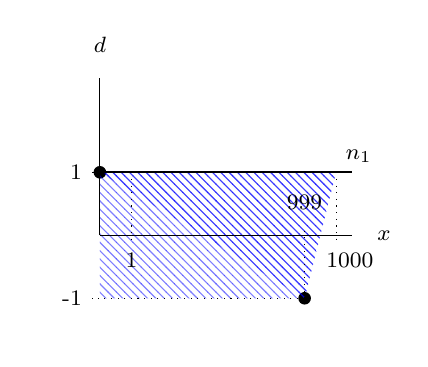
\begin{tikzpicture}[y=.2cm, x=.2cm,font=\footnotesize]

	\fill<-1>[line] (0,4) circle (0.4);
	\fill<6-8>[line] (13,-4) circle (0.4);
	\fill<7>[polyhedra] (13,-4) -- (0,4) -- (15,4) -- cycle;
	\fill<8>[polyhedra] (13,-4) -- (0,-4) -- (0,4) -- (15,4) -- cycle;
	\draw<3>[line] (0,4) -- (2,4) -- cycle;
	\draw<2>[line] (0,4) -- (16,4) -- cycle;
	\draw<4>[line] (0,4) -- (16,4) -- cycle;
	\draw<5->[line] (0,4) -- (15,4) -- cycle;

 	%axis
	\draw (0,0) -- coordinate (x axis mid) (16,0);
    \draw (0,0) -- coordinate (y axis mid) (0,10);

	%ticks and labels      
	\node[right=1.8cm] at (x axis mid) {$x$};
	\node[above=1.2cm] at (y axis mid) {$d$};
	
	\node at (-4,-6) {};

     		\draw<1-> (1pt,4) -- (-3pt,4) 
     			node[anchor=east] {1}; 
     		\draw<6-> [dotted] (13,-4) -- (-3pt,-4) 
     			node[anchor=east] {-1}; 
     		\draw<3-3> [dotted] (2,4) -- (2,-3pt) 
     			node[anchor=north] {1}; 
     		\draw<5-> [dotted] (15,4) -- (15,-3pt) 
     			node[anchor=north,xshift=5pt] {1000}; 
     		\draw<6-> [dotted] (13,-4) -- (13,3pt) 
     			node[anchor=north,yshift=15pt] {999}; 

	\node[right=3cm] at (y axis mid) {$n_1$};
\end{tikzpicture} 
\end{column}
\end{columns}
\end{frame}


\section[Combining both techniques]{Combining Both Techniques}

\begin{frame}
	\frametitle{Principle}
	
	\begin{center}
	We apply Guided Static Analysis over the Reduced Multigraph
	\end{center}
	\vspace{1cm}
	
	$\Rightarrow$ Ascending sequence of subset of paths
	
\end{frame}

\begin{frame}
	\frametitle{Algorithm}
	3 phases:
	\begin{enumerate}
		\item Compute new feasible paths
		\item Path Focusing on the subset of the multigraph
		\item Narrowing iterations
	\end{enumerate}

	\begin{center}
	and restart\ldots
	\end{center}

	\begin{itemize}
		\item We maintain a set $P$ of paths : subgraph we are working on
	\end{itemize}
\end{frame}

\begin{frame}
	\frametitle{Computing New Paths}

New feasible paths starting from $p_1$:
\begin{figure}[!h]
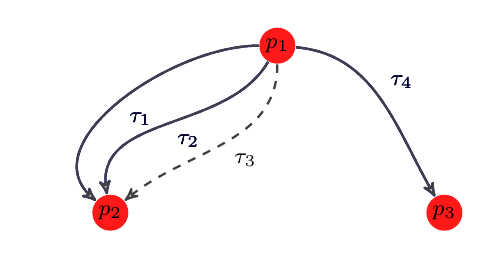
\begin{tikzpicture}[->,>=stealth',auto,node distance=3cm,
                    semithick,font=\footnotesize]

	\node[PRstate] (n0) {$p_1$};
	\node[PRstate] (n2) [below left of=n0] {$p_2$};
	\node[PRstate] (n3) [below right of=n0] {$p_3$};

	\path [NewPath] 
		(n0) edge  [out=-90, in=40]            node {$\tau_3$} (n2);

	\path<-3> [NewPath] 
		(n0) edge  [out=-120, in=100]            node {$\tau_2$} (n2);
	\path<4> [TakenPath] 
		(n0) edge  [out=-120, in=100]            node {$\tau_2$} (n2);
	\path<5-> [transition] 
		(n0) edge  [out=-120, in=100]            node {$\tau_2$} (n2);
  
	\path<1> [NewPath] 
		(n0) edge  [out=180, in=140]            node {$\tau_1$} (n2);
	\path<2> [TakenPath] 
		(n0) edge  [out=180, in=140]            node {$\tau_1$} (n2);
	\path<3-> [transition] 
		(n0) edge  [out=180, in=140]            node {$\tau_1$} (n2);
  
	\path<-2> [NewPath] 
		(n0) edge  [out=-5, in=120]            node {$\tau_4$} (n3);
	\path<3> [TakenPath] 
		(n0) edge  [out=-5, in=120]            node {$\tau_4$} (n3);
	\path<4-> [transition] 
		(n0) edge  [out=-5, in=120]            node {$\tau_4$} (n3);
\end{tikzpicture}
\end{figure}
$p_2 : X_2 \visible<2->{\sqcup \tau_1(X_1)} \visible<4->{\sqcup \tau_2(X_1)}$
\hfill 
$p_3 : X_3 \visible<3->{\sqcup \tau_4(X_1)}$

\vspace{0.5cm}
\visible<5->{
$\tau_3$ feasible, but:
$$\tau_3(p_1) \subset X_2 \sqcup \tau_1(X_1) \sqcup \tau_2(X_1)$$
}
\end{frame}

\begin{frame}
	\frametitle{Ascending iterations}

	Path Focusing algorithm on the multigraph

	\vspace{1cm}	

	But the formula is cunjunct with $P$ (subgraph): 
	$$f(p_i) \wedge P$$

	\vspace{1cm}
	\visible<2->{
	We also cunjunct the formula with $P$ for narrowing iterations\ldots
	}
\end{frame}

%\begin{frame}
%	\frametitle{Example}
%
%\begin{figure}[!h]
%\begin{tikzpicture}[->,>=stealth',auto,node distance=1.5cm,
%                    semithick,font=\footnotesize]
%	\node[PRstate] (n0) {$n_0$};
%	\node[PRstate] (n1) [below of=n0] {$n_1$};
%	\node[PRstate] (n9) [below of=n1,yshift=-4cm] {$n_9$};
%
%  \path [transition] 
%		(n0) edge              node  {$\begin{array}{l}
%		x \leftarrow 0 \\
%		d \leftarrow 1 
%		\end{array}$} (n1);
%  \path<4-> [transition] 
%        (n1)  edge [out=-160,in=160]  node [left,xshift=0.2cm] {$\begin{array}{l} 0< x < 1000/\end{array}$} (n9);
%  \path<2-> [transition] 
%        (n1)  edge [out=-90,in=90]  node [xshift=-0.2cm] {$\begin{array}{l} x = 0/ \\ d \gets 1\end{array}$} (n9);
%  \path<5-> [transition] 
%        (n1)  edge [out=-20,in=20]  node [right,xshift=-0.2cm] {$\begin{array}{l}  x = 1000/ \\ d \gets -1\end{array}$} (n9);
%  \path<3-> [transition] 
%        (n9) edge [out=0, in=0, distance=4.3cm] node [right] {$x \leftarrow x+d$} (n1);
%\end{tikzpicture}
%\end{figure}
%\end{frame}

\section{Computing Disjunctive Invariants}

\begin{frame}
	\frametitle{Extending Gulwani et al's technique (1)}
	Example:
\begin{center}
\tikzstyle{associate}=[draw, dashed]

\tikzstyle{invariant}=[regular polygon,regular polygon sides=5,fill=black!25,minimum size=13pt,inner sep=0pt]
% Everything is drawn on underlying gray rectangles with
% rounded corners.
\tikzstyle{background}=[rectangle,
                                                fill=gray!10,
                                                inner sep=0.2cm,
                                                rounded corners=5mm]

\begin{tikzpicture}[>=stealth',auto,node distance=1.1cm,
                    semithick,font=\footnotesize]

	\node[invariant] (n1) {$X_1$};
	\node[invariant] (n2) [below of=n1] {$X_2$};
	\node[invariant] (n3) [below of=n2] {$X_3$};
	\node[invariant] (n4) [below of=n3] {$X_4$};
	\node[invariant] (n5) [below of=n4] {$X_5$};

	\node (p1) [above right of=n1, xshift=1.3cm] {};
	\node (p2) [below of=p1] {};
	\node (p3) [below of=p2] {};
	\node (p4) [below of=p3] {};
	\node (p5) [below of=p4] {};
	\node (p6) [below of=p5] {};

	\node (P1) [right of=p1, xshift=0.5cm] {};
	\node (P2) [right of=p2, xshift=0.5cm] {};
	\node (P3) [right of=p3, xshift=0.5cm] {};
	\node (P4) [right of=p4, xshift=0.5cm] {};
	\node (P5) [right of=p5, xshift=0.5cm] {};
	\node (P6) [right of=p6, xshift=0.5cm] {};

	\node[invariant] (N1) [below right of=P1, xshift=2cm, yshift=-0.5cm] {$Y_1$};
	\node[invariant] (N2) [below of=N1] {$Y_2$};
	\node[invariant] (N3) [below of=N2] {$Y_3$};
	\node[invariant] (N4) [below of=N3] {$Y_4$};

 \path [transition] 
		(p1) edge              node {$\tau_1$} (P1);
 \path [transition] 
		(p2) edge              node {$\tau_2$} (P2);
 \path [transition] 
		(p3) edge              node {$\tau_3$} (P3);
 \path [transition] 
		(p4) edge              node {$\tau_4$} (P4);
 \path [transition] 
		(p5) edge              node {$\tau_5$} (P5);
 \path [transition] 
		(p6) edge              node {$\tau_6$} (P6);

 \path<2> [associate] (n1) -- (p1);
 \path<2> [associate] (P1) -- (N2);

 \path<3> [associate] (n1) -- (p2);
 \path<3> [associate] (P2) -- (N4);

 \path<5> [associate] (n2) -- (p3);
 \path<5> [associate] (P3) -- (N4);

 \path<4> [associate] (n2) -- (p2);
 \path<4> [associate] (P2) -- (N1);

 \begin{pgfonlayer}{background}
        \node [background,
                    fit=(n1) (n5),
					label=below:\begin{tabular}{c}Source \\
						Invariant\end{tabular}] {};
        \node [background,
                    fit=(p1) (P6),
                    label=below:Paths] {};
        \node [background,
                    fit=(N1) (N4),
					label=below:\begin{tabular}{c}Destination \\
						Invariant\end{tabular}] {};
  \end{pgfonlayer}
\end{tikzpicture}
\end{center}
\end{frame}

\begin{frame}
	\frametitle{Extending Gulwani et al's technique (2)}

Disjunctive invariant for $p_i$ : $\bigvee_{1\leq j \leq m_i} X_{i,j}$

\begin{itemize}
	\item $\delta_i \in [1,m_i]$
	\item mapping function $\sigma_i: [1,m_i] \times [1,n_i] \mapsto [1,m_i]$
\end{itemize}

\vspace{1cm}

$X_{i,\delta_i} \gets$ initial states

\vspace{0.4cm}

The image of the $j$-th disjunct $X_{i,j}$ by the $k$-th path $\tau_{i,k}$ is
joined with $X_{i,\sigma_i(j,k)}$.
\end{frame}

\begin{frame}
	\frametitle{Extending Gulwani et al's technique (3)}

We extend our SMT formula to handle disjunctive invariants:

\begin{eqnarray*}
g(p_i) & = & \rho \wedge b_i^s \wedge 
\displaystyle\bigwedge_{j \in P_R \atop j \neq i} \neg b_j^s  \\
 & & \wedge 
\important{\displaystyle\bigvee_{1 \leq k \leq m_i} (d_k \wedge X_{i,k} \wedge \bigwedge_{l \neq k}
\neg d_l)} \\
 & & \wedge
\displaystyle\bigvee_{j \in Succ(i)} 
(b_j^d \wedge \important{\bigwedge_{1 \leq k \leq m_i} (\neg X_{j,k})})
\end{eqnarray*}

In the model, $d_k = true \implies$ we use $X_{i,k}$ as the starting disjunct.
\end{frame}

\begin{frame}
	\frametitle{Dynamic construction of $\sigma$}

	$M$: maximum number of disjunct

	$m_i$: current number of disjunct

	\vspace{1cm}
When $\sigma_i(j,k)$ is undefined:
\begin{enumerate}
	\item if $\exists j', \tau_{i,k}(X_{i,j}) \sqcup X_{i',j'} =
		\tau_{i,k}(X_{i,j}) \cup X_{i',j'}$, we assign $\sigma_i(j,k)$ to $j'$
	\item else:
	\begin{itemize}
		\item if $m_i < M$, we increment $m_i$ and define $\sigma_i(j,k) = m_i$
		\item if $m_i = M$, we define $\sigma_i(j,k) = M$ 
	\end{itemize}
\end{enumerate}
\end{frame}

\begin{frame}[containsverbatim]
	\frametitle{Example}
\begin{center}
\begin{lstlisting}
	int x = 0;
	int d = 1;
	
	while (true) {
		if (x == 0) d=1;
		if (x == 1000) d=-1;
		x +=d;
	}
\end{lstlisting}
\end{center}
We find:
$$(d = 1 \wedge 0 \leq x \leq 1000) \vee
(d = -1 \wedge 0 \leq x \leq 999)$$
\end{frame}

\begin{frame}
	\frametitle{Experiments}
	These techniques are implemented in a prototype of static analyzer:
	\begin{itemize}
		\item LLVM IR as input
		\item Apron Library
		\item Microsoft Z3, Yices
	\end{itemize}
\end{frame}

\begin{frame}
\begin{figure}[h]
  \begin{center}
    % GNUPLOT: LaTeX picture with Postscript
\begingroup
  \makeatletter
  \providecommand\color[2][]{%
    \GenericError{(gnuplot) \space\space\space\@spaces}{%
      Package color not loaded in conjunction with
      terminal option `colourtext'%
    }{See the gnuplot documentation for explanation.%
    }{Either use 'blacktext' in gnuplot or load the package
      color.sty in LaTeX.}%
    \renewcommand\color[2][]{}%
  }%
  \providecommand\includegraphics[2][]{%
    \GenericError{(gnuplot) \space\space\space\@spaces}{%
      Package graphicx or graphics not loaded%
    }{See the gnuplot documentation for explanation.%
    }{The gnuplot epslatex terminal needs graphicx.sty or graphics.sty.}%
    \renewcommand\includegraphics[2][]{}%
  }%
  \providecommand\rotatebox[2]{#2}%
  \@ifundefined{ifGPcolor}{%
    \newif\ifGPcolor
    \GPcolorfalse
  }{}%
  \@ifundefined{ifGPblacktext}{%
    \newif\ifGPblacktext
    \GPblacktexttrue
  }{}%
  % define a \g@addto@macro without @ in the name:
  \let\gplgaddtomacro\g@addto@macro
  % define empty templates for all commands taking text:
  \gdef\gplbacktext{}%
  \gdef\gplfronttext{}%
  \makeatother
  \ifGPblacktext
    % no textcolor at all
    \def\colorrgb#1{}%
    \def\colorgray#1{}%
  \else
    % gray or color?
    \ifGPcolor
      \def\colorrgb#1{\color[rgb]{#1}}%
      \def\colorgray#1{\color[gray]{#1}}%
      \expandafter\def\csname LTw\endcsname{\color{white}}%
      \expandafter\def\csname LTb\endcsname{\color{black}}%
      \expandafter\def\csname LTa\endcsname{\color{black}}%
      \expandafter\def\csname LT0\endcsname{\color[rgb]{1,0,0}}%
      \expandafter\def\csname LT1\endcsname{\color[rgb]{0,1,0}}%
      \expandafter\def\csname LT2\endcsname{\color[rgb]{0,0,1}}%
      \expandafter\def\csname LT3\endcsname{\color[rgb]{1,0,1}}%
      \expandafter\def\csname LT4\endcsname{\color[rgb]{0,1,1}}%
      \expandafter\def\csname LT5\endcsname{\color[rgb]{1,1,0}}%
      \expandafter\def\csname LT6\endcsname{\color[rgb]{0,0,0}}%
      \expandafter\def\csname LT7\endcsname{\color[rgb]{1,0.3,0}}%
      \expandafter\def\csname LT8\endcsname{\color[rgb]{0.5,0.5,0.5}}%
    \else
      % gray
      \def\colorrgb#1{\color{black}}%
      \def\colorgray#1{\color[gray]{#1}}%
      \expandafter\def\csname LTw\endcsname{\color{white}}%
      \expandafter\def\csname LTb\endcsname{\color{black}}%
      \expandafter\def\csname LTa\endcsname{\color{black}}%
      \expandafter\def\csname LT0\endcsname{\color{black}}%
      \expandafter\def\csname LT1\endcsname{\color{black}}%
      \expandafter\def\csname LT2\endcsname{\color{black}}%
      \expandafter\def\csname LT3\endcsname{\color{black}}%
      \expandafter\def\csname LT4\endcsname{\color{black}}%
      \expandafter\def\csname LT5\endcsname{\color{black}}%
      \expandafter\def\csname LT6\endcsname{\color{black}}%
      \expandafter\def\csname LT7\endcsname{\color{black}}%
      \expandafter\def\csname LT8\endcsname{\color{black}}%
    \fi
  \fi
  \setlength{\unitlength}{0.0500bp}%
  \begin{picture}(5040.00,5040.00)%
    \gplgaddtomacro\gplbacktext{%
      \csname LTb\endcsname%
      \put(594,966){\makebox(0,0)[r]{\strut{} 0}}%
      \put(594,1442){\makebox(0,0)[r]{\strut{} 2}}%
      \put(594,1918){\makebox(0,0)[r]{\strut{} 4}}%
      \put(594,2394){\makebox(0,0)[r]{\strut{} 6}}%
      \put(594,2871){\makebox(0,0)[r]{\strut{} 8}}%
      \put(594,3347){\makebox(0,0)[r]{\strut{} 10}}%
      \put(594,3823){\makebox(0,0)[r]{\strut{} 12}}%
      \put(594,4299){\makebox(0,0)[r]{\strut{} 14}}%
      \put(594,4775){\makebox(0,0)[r]{\strut{} 16}}%
      \put(1216,834){\rotatebox{-45}{\makebox(0,0)[l]{\strut{}G/S}}}%
      \put(1705,834){\rotatebox{-45}{\makebox(0,0)[l]{\strut{}PF/S}}}%
      \put(2195,834){\rotatebox{-45}{\makebox(0,0)[l]{\strut{}PF/G}}}%
      \put(2685,834){\rotatebox{-45}{\makebox(0,0)[l]{\strut{}G+PF/PF}}}%
      \put(3174,834){\rotatebox{-45}{\makebox(0,0)[l]{\strut{}G+PF/G}}}%
      \put(3664,834){\rotatebox{-45}{\makebox(0,0)[l]{\strut{}G+PF/S}}}%
      \put(4153,834){\rotatebox{-45}{\makebox(0,0)[l]{\strut{}DIS/G+PF}}}%
      \put(236,2871){\rotatebox{-270}{\makebox(0,0){\strut{}percentage of control points}}}%
    }%
    \gplgaddtomacro\gplfronttext{%
      \put(3656,4602){\makebox(0,0)[r]{\strut{}$\subsetneq$}}%
      \put(3656,4382){\makebox(0,0)[r]{\strut{}$\supsetneq$}}%
      \put(3656,4162){\makebox(0,0)[r]{\strut{}uncomparable}}%
    }%
    \gplbacktext
    \put(0,0){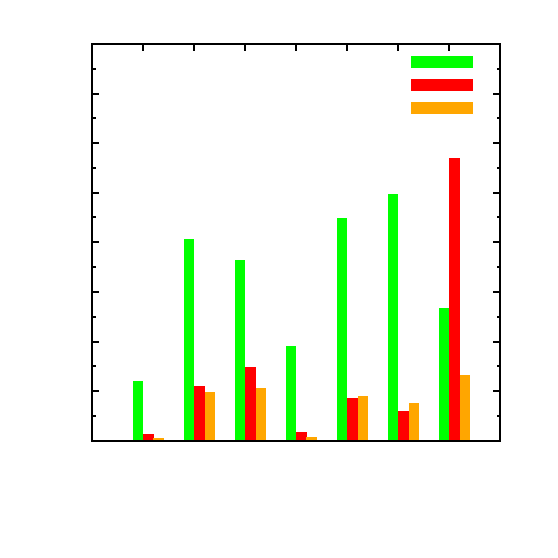
\includegraphics{gnuplot/techniques}}%
    \gplfronttext
  \end{picture}%
\endgroup

  \end{center} 
  \end{figure}
\end{frame}

\begin{frame}
	\frametitle{Time}
\begin{table}[!h]
	\centering
\begin{tabular}{|l|r|r|r|r|r|} \hline
	\multicolumn{1}{|c|}{Benchmark} &
		\multicolumn{1}{c|}{\textbf{S}} &
		\multicolumn{1}{c|}{\textbf{G}} &
		\multicolumn{1}{c|}{\textbf{PF}} &
		\multicolumn{1}{c|}{\textbf{G+PF}} &
	\multicolumn{1}{c|}{\textbf{DIS}} \\ \hline
a2ps-4.14 & 64 & 17 & 66 & 175 & 512 \\
gawk-4.0.0 & 59 & 8 & 18 & 43 & 129 \\
gnuchess-6.0.0 & 112 & 21 & 122 & 374 & 866 \\
gnugo-3.8 & 155 & 31 & 128 & 382 & 1403 \\
grep-2.9 & 50 & 12 & 21 & 58 & 307 \\
gzip-1.4 & 63 & 12 & 36 & 97 & 617 \\
lapack-3.3.1 & 721 & 246 & 2690 & 6052 & 22222 \\
make-3.82 & 22 & 7 & 32 & 83 & 255 \\
sed-4.2 & 35 & 7 & 23 & 69 & 521 \\
tar-1.26 & 270 & 39 & 110 & 304 & 1164 \\
	\hline
\end{tabular}
\caption{Execution time for each technique, expressed in seconds}
\label{tab:time}
\end{table}

\end{frame}

\begin{frame}
\begin{center}
Thank you.
\end{center}
\end{frame}

\end{document}

%%% Local Variables:
%%% mode: latex
%%% TeX-master: t
%%% ispell-local-dictionary: "american"
%%% End:
